\documentclass[tikz,border=12pt]{standalone}
\usepackage{amsmath,amssymb}
\usetikzlibrary{calc,arrows.meta}

\begin{document}
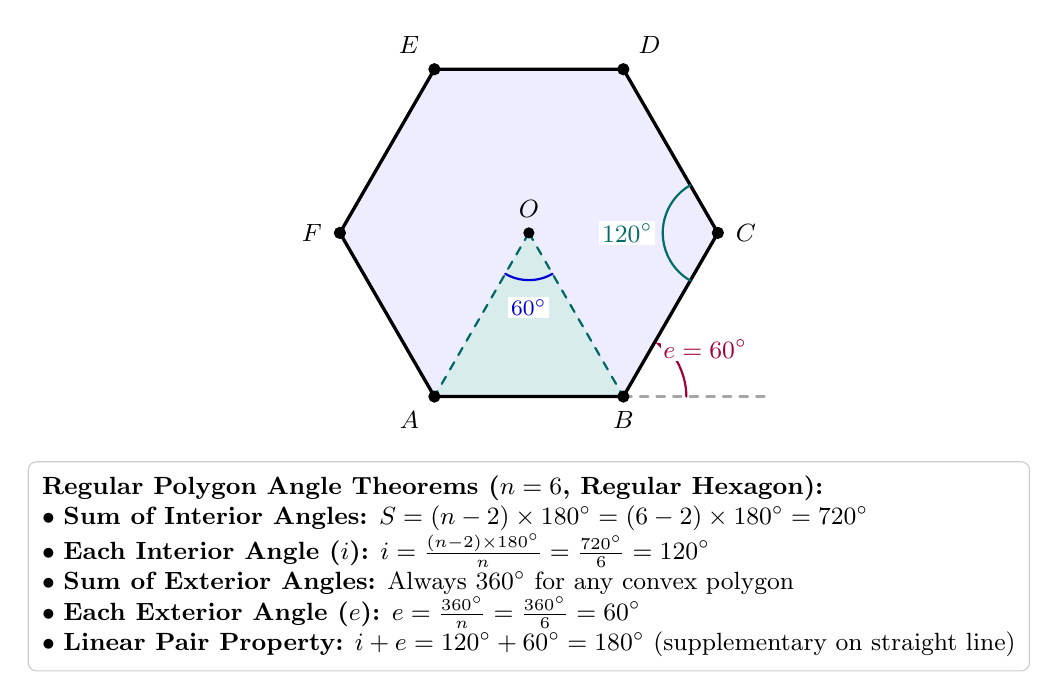
\begin{tikzpicture}[>=latex, line cap=round, line join=round]

  % Parameters for regular hexagon (radius R = 2.4)
  \def\R{2.4}

  % Coordinates of hexagon vertices
  \coordinate (O) at (0, 0);
  \coordinate (A) at (240:\R);
  \coordinate (B) at (300:\R);
  \coordinate (C) at (0:\R);
  \coordinate (D) at (60:\R);
  \coordinate (E) at (120:\R);
  \coordinate (F) at (180:\R);

  % Hexagon body shading
  \fill[blue!7] (A) -- (B) -- (C) -- (D) -- (E) -- (F) -- cycle;

  % Central triangle OAB highlighted
  \fill[teal!15] (O) -- (A) -- (B) -- cycle;
  \draw[thick, dashed, teal!80!black] (O) -- (A);
  \draw[thick, dashed, teal!80!black] (O) -- (B);

  % Hexagon boundary
  \draw[very thick] (A) -- (B) -- (C) -- (D) -- (E) -- (F) -- cycle;

  % Collinear baseline extension of side AB past B to show exterior angle
  \draw[thick, dashed, gray!70] (B) -- ++(1.8, 0) coordinate (X);

  % Exterior angle arc at B (from 0 deg up to 60 deg -> sweep 60 deg)
  \draw[thick, ->, purple!85!black] ([shift=(0:0.8)]B) arc[start angle=0, delta angle=60, radius=0.8];
  \node[font=\small\bfseries, purple!85!black, fill=white, inner sep=1pt] at ($(B) + (30:1.2)$) {$e = 60^\circ$};

  % Interior angle arc at vertex C (from 120 deg to 240 deg -> sweep 120 deg)
  \draw[thick, teal!85!black] ([shift=(120:0.7)]C) arc[start angle=120, delta angle=120, radius=0.7];
  \node[font=\small\bfseries, teal!85!black, fill=white, inner sep=1pt] at ($(C) + (180:1.15)$) {$120^\circ$};

  % Central angle arc at O
  \draw[thick, blue!85!black] ([shift=(240:0.6)]O) arc[start angle=240, delta angle=60, radius=0.6];
  \node[font=\footnotesize\bfseries, blue!85!black, fill=white, inner sep=1pt] at ($(O) + (270:0.95)$) {$60^\circ$};

  % Vertices
  \filldraw[black] (O) circle (1.8pt) node[above=2pt, font=\small\bfseries] {$O$};
  \filldraw[black] (A) circle (2pt) node[below left=2pt, font=\small\bfseries] {$A$};
  \filldraw[black] (B) circle (2pt) node[below=2pt, font=\small\bfseries] {$B$};
  \filldraw[black] (C) circle (2pt) node[right=3pt, font=\small\bfseries] {$C$};
  \filldraw[black] (D) circle (2pt) node[above right=2pt, font=\small\bfseries] {$D$};
  \filldraw[black] (E) circle (2pt) node[above left=2pt, font=\small\bfseries] {$E$};
  \filldraw[black] (F) circle (2pt) node[left=3pt, font=\small\bfseries] {$F$};

  % Summary Card below
  \node[align=left, font=\small, fill=white, inner sep=5pt, draw=gray!40, rounded corners=3pt, anchor=north] at (0, -2.9) {
    \textbf{Regular Polygon Angle Theorems ($n = 6$, Regular Hexagon):}\\
    $\bullet$ \textbf{Sum of Interior Angles:} $S = (n - 2) \times 180^\circ = (6 - 2) \times 180^\circ = 720^\circ$\\
    $\bullet$ \textbf{Each Interior Angle ($i$):} $i = \frac{(n - 2) \times 180^\circ}{n} = \frac{720^\circ}{6} = 120^\circ$\\
    $\bullet$ \textbf{Sum of Exterior Angles:} Always $360^\circ$ for any convex polygon\\
    $\bullet$ \textbf{Each Exterior Angle ($e$):} $e = \frac{360^\circ}{n} = \frac{360^\circ}{6} = 60^\circ$\\
    $\bullet$ \textbf{Linear Pair Property:} $i + e = 120^\circ + 60^\circ = 180^\circ$ (supplementary on straight line)
  };

\end{tikzpicture}
\end{document}
